\documentclass[12pt]{article}

\usepackage[francais]{babel}
\usepackage[T1]{fontenc}
\usepackage[utf8]{inputenc}
\usepackage{graphicx}
\usepackage{hyperref}
\usepackage{listings}
\usepackage{pgfgantt}
\usepackage{diagbox}
\usepackage{tikz}
\usepackage{array}
\usetikzlibrary{calc,positioning,arrows}
\usepackage{float}

\usepackage{tikz}
\usepackage{pgfplots}
\pgfplotsset{compat=1.14}
\usepackage{amssymb}
\usepackage{amsmath}

\title{PDP: Reversi\\Mémoire}
\author{
  Chemoune Alaeddine\\ 
  \and
  Delengaigne Hadrien\\
  \and
  Pivetaud Victor\\
  \and
  Schlick Charlie\\
}

\begin{document}
\maketitle

\tableofcontents

\section{Introduction}
Le \textit{Reversi} est un jeu de société qui se joue à deux joueurs, avec des pions noirs et blancs, sur un plateau composé de 64 cases. Ce jeu est apparu en 1883 en Angleterre sous le nom de \textit{Reversi}, mais son invention reste contestée. La version moderne est connue sous le nom d'\textit{Othello} et a été brevetée en 1971 au Japon par \textit{Goro Hasegawa} et diffère légèrement de son ancêtre, notamment par le placement des pions en début de partie\cite{othello}(les joueurs plaçaient chacun à son tour les pions de départ sur les 4 cases centrales, ce qui pouvait aboutir à la même configuration que l'Othello ou à une configuration avec les pions blancs et noirs en parallèle). Depuis 1977 un championnat du monde est organisé chaque année. Les sommaires règles de base offrent la possibilité aux meilleurs joueurs de prévoir plusieurs coups à l'avance, ce qui permet de développer des stratégies complexes. 

Au début d'une partie, quatre pions sont posés au centre du plateau, deux faces blanches et deux faces noires en diagonale. Le but du jeu est d'avoir le plus de pions de sa couleur. Pour prendre des pièces à son adversaire, il faut mettre ses pions aux extrémités d'une ligne de pions adverses. Chaque joueur pose donc un nouveau pion sur le plateau à chaque tour. Seuls les coups qui permettent de prendre au moins une pièce à l'adversaire sont autorisés. La partie se termine lorsque le plateau est plein ou lorsque plus aucun coup n'est jouable, le gagnant est alors le joueur qui possède le plus de pions de sa couleur sur le plateau.

\section{Description et analyse de l'existant}

De nombreux programmes de \textit{Reversi} ont été développés et déjà avant la défaite du champion Takeshi Murakami contre le programme Logistello en 1997(avec un score de 6-0) on pouvait affirmer que les programmes étaient meilleurs que les humains à ce jeu. La grande problématique de recherche sur les jeux de plateau est de parvenir à les résoudre. On génère un arbre dont les sommets représentent les états du jeu et les chemins des coups possibles (il est aussi nécessaire de noter qui doit jouer dans le cas où un des joueurs est forcé de passer son tour). On va ainsi pouvoir représenter tous les enchaînements de coups. Résoudre un jeu signifie que l'on est capable d'aller au bout de l'arbre, ainsi on est toujours capable de contrer l'adversaire. Cela ne veut pas dire que l'on a parcouru tous les sommets, on peut simplifier l'arbre représentant tous les coups (par exemple dans le Reversi les 4 possibles sont symétriques, la position choisie n'importe pas et on peut donc ne regarder qu'un seul des 4 sous-arbres).
\begin{figure}[H]
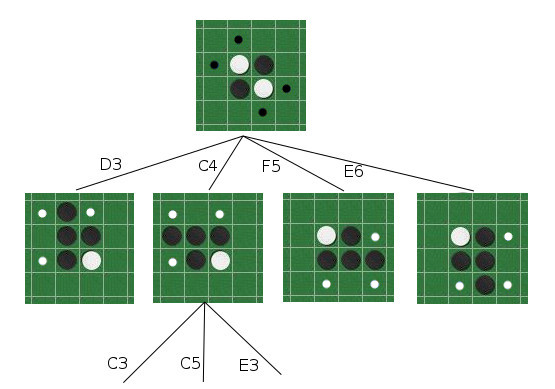
\includegraphics[scale=0.6]{exemple_arbre.jpg}
\centering
\caption{Exemple d'arbre que l'on peut générer. A partir de la position de départ du jeu, les sommets de l'arbre sont les états et les chemins des coups possibles.}
\label{config_depart}
\end{figure}

\subsection{Techniques de parcours d'arbres:}
Même si le \textit{Reversi} sur un plateau de 8x8 n'a pas encore été résolu, des solutions ont été trouvées pour des parties en 4x4 et 6x6\cite{sol6x6}.

Afin de trouver rapidement le meilleur coup (celui qui donne le plus de chance de gagner la partie), les programmes ont besoin dans un premier temps d'une technique de parcours d'arbre efficace, mais aussi d'heuristique. De nombreuses techniques de parcours existent, parmi les plus utilisées on peut citer:
\begin{itemize}
\item \textit{Minimax Alpha-beta pruning}\cite{alpha-beta}, le grand avantage de cette méthode est qu'elle élimine des branches au fur et à mesure de son déroulement. Elle est donc assez optimisée pour les arbres représentant les coups possibles d'un jeu de plateau.
\item \textit{Negamax} Une variante simplifiée de minimax, lors du calcul de la perte maximale on part du principe que la valeur d'un coup pour un joueur donné est égale à la négation de la valeur de l'autre joueur. Ainsi au lieu de calculer le minimum et maximum pour chaque joueur et chaque coup on dit que \begin{math}
max(a, b) == -min(-a, -b).
\end{math}
\item \textit{Monte Carlo tree search}\cite{MonteCarlo} Le but est de jouer des parties aléatoirement pour étudier la probabilité de gagner d'une configuration. Pour cela il parcourt l'arbre des coups qu'il a déjà créé en choisissant le meilleur nœud parmi les candidats et re-simule à partir du meilleur nœud connu pour mettre à jour les probabilités. 
\end{itemize}

\subsection{Les fonctions d'évaluation:}
Comme dit précédemment, on ne sait pas, à l'heure actuelle, aller jusqu'au bout de l'arbre des coups possibles, c'est la raison pour laquelle nous avons besoin d'une fonction d'évaluation. Le but de cette fonction est d'attribuer une valeur aux sommets représentant les états du jeu. Pour se faire, plusieurs techniques sont possibles\cite{heuristique}.
\begin{itemize}
\item IAGO: Cette méthode consiste à utiliser les connaissances que l'on a du jeu de Reversi\cite{strategie}, en effet on peut dégager des critères augmentant les chances de gagner. Par exemple les bords et les coins sont des positions très intéressantes à avoir car elles sont difficiles ou impossibles à retourner. En réduisant le nombre de coups possibles pour l'adversaire on peut aussi l'obliger à jouer des coups nous favorisant (par exemple nous permettre de prendre possession d'un coin). En étant capable d'extraire ces informations on peut évaluer chaque coup.
\item LOGISTELLO: La méthode utilisée par le programme ayant battu le champion du monde se base sur des parties jouées. En faisant analyser les coups joués et le résultat de la partie à un ordinateur on peut obtenir une heuristique basée sur des parties réelles plutôt que deviner les éléments importants pour gagner.
\end{itemize}

\medbreak
De grand progrès sont actuellement en cours dans le secteur des intelligences artificielles grâce au machine learning. Le but est de fournir de nombreuses données à la machine afin qu'elle apprenne seule. C'est cette technique qui a permis de créer une IA surpassant l'humain au jeu de Go. La méthode consistant à créer un arbre de recherche comprenant les coups possibles énoncés précédemment n'est pas applicable au jeu de Go, en effet sa complexité spatiale (le nombre de configuration de partie possible) est plus d'un gogol
(\begin{math}
10^{100}
\end{math})
fois plus grand que le jeu d'échec.

L'IA AlphaGo\cite{AlphaGo} utilise l’algorithme de parcours d'arbre "Monte Carlo" en combinaison avec deux réseaux de neurone (un réseau de valeur trouvant la probabilité de gagner sans devoir parcourir tout l'arbre et un réseau d'objectif filtrant les coups inutiles). Cette version d'AlphaGo utilisais les données extraites de milliers de parties jouées entre humains.

Son évolution AlphaGo Zero\cite{AlphaGoZero} utilise des données obtenues à partir de partie jouée contre lui même, cette différence permet de dépasser les connaissances humaines. En 40 jours d'apprentissage AlphaGo Zero dépasse toutes les versions précédentes.

\medbreak
Enfin, afin de représenter le plateau d'une façon permettant des manipulations rapides, une structure spécifique a été inventée: les Bitboards\cite{bitboard}. Cette structure de données est un tableau de bit représentant la présence ou non des pions sur la case correspondante. Le principal avantage de cette stucture est qu'elle permet la manipulation du plateau par des opérations bit à bit, opérations pouvant être effectuées très rapidement par les processeurs. Le deuxième avantage est que cette information prend très peu de place en mémoire. Dans le cas du Reversi, le plateau peut être représenté par deux bitboards, un codant les positions des pions blancs et l'autre les positions des pions noirs.



\section{Description des besoins}
\subsection{Fonctionnels}

\subsubsection{Liste des besoins liés à la simulation de jeu :}

\textbf{Déterminer les coups possibles à jouer :}
Dans les règles du Reversi\cite{regle}, tous les coups ne sont pas possibles, il est même possible que aucun coup ne le soit, nous devons donc pouvoir les déterminer à chaque tour pour respecter les règles du jeu et pour savoir si le coup qui est demandé est légal ou non.

\textbf{Actualiser le plateau après un coup :}
L'action de poser un pion sur le plateau entraine la capture de un ou plusieurs pion(s) du joueur adverse, il faut donc mettre à jour l'état du plateau avant de changer de joueur.

\textbf{Reconnaître une fin de partie : }
Pour savoir quand arrêter le jeu nous devons reconnaître une fin de partie. Il n'y a soit plus de case libre soit plus de coups légaux disponibles pour les deux joueurs.

\subsubsection{Liste des besoins liés à l'interface utilisateur :}

\textbf{Démarrer une partie :}
Au lancement du programme il faut qu'une partie se lance selon les paramètres passés par l'utilisateur, ces options permettront de:
\begin{itemize}
\item spécifier la taille
\item reprendre une partie sauvegardée dans un fichier texte
\item faire jouer les blancs et/ou noirs par une IA
\item lancer le mode contest
\item afficher l'aide
\end{itemize}

\textbf{Afficher l'état de la partie sur la console :}
Il faut pouvoir afficher le plateau de jeu quelle que soit sa taille, en dessous d'une certaine limite, et d'une manière qui soit compréhensible par le joueur.

\textbf{Déterminer les coups possibles à jouer et les afficher:}
Il faut pouvoir prévoir les coups légaux qui permettent de prendre des pions à l'adversaire et les rajouter sur l’affichage, pour que le joueur puisse savoir où il a le droit de jouer.

\textbf{Choisir un coup:}
Le joueur doit pouvoir placer un pion, ce qui aura pour effet si le coup est légal, d'actualiser l’état de la partie, ou le cas échéant, de redemander une position au joueur.

\textbf{Terminer une partie : }
La partie se terminera par un affichage des scores et la possibilité de recommencer une partie, ou d’arrêter le programme sera proposée au joueur.

\textbf{Sauvegarder une partie dans un fichier texte :} 
Si l'on souhaite continuer la partie plus tard, nous devons être capables de quitter le jeu à tout moment en tapant 'q' au lieu de choisir un coup et sauvegarder l'état actuel dans un simple fichier texte avant de fermer le programme. L'écriture de ce fichier doit respecter la syntaxe fixée par le client (Voir figure ~\ref{SaveExemple}) qui sera expliquée plus bas.

\textbf{Charger une partie à partir d'un fichier de sauvegarde :}
Une fois qu'une partie est sauvegardée, si l'on souhaite la continuer nous devons pouvoir placer en entrée de notre programme le nom d'un fichier de sauvegarde qui respecte la syntaxe (voir figure ~\ref{SaveExemple}) et continuer la partie à partir de l'état de jeu actuel.

\textbf{Respecter la syntaxe du fichier de sauvegarde (voir figure ~\ref{SaveExemple}) pour que le programme arbitre du client puisse l'utiliser :}

\begin{itemize}
\item Les lignes vides, espaces et tabulation ne sont pas pris en compte, seuls les lignes non vides sont significatives.
\item La première ligne significative indique le joueur courant('X' pour le joueur noir et 'O' pour le joueur blanc).
\item Chaque ligne significative qui suit représente une ligne du plateau, avec pour chaque case,'\_' si la case est vide, 'X' si il y a un pion noir et 'O' si il y a un pion blanc.
\item Chaque fin de ligne est définie par un '\textbackslash n'.
\item Le caractère '\#' indique un commentaire jusqu'au prochain '\textbackslash n'
\item Les lignes ne contenant que des commentaires sont donc des lignes considérées vides.
\item Il faut respecter les tailles carrées et paires telles que 2x2, 4x4, 6x6, 8x8...
\end{itemize}
\begin{figure}[H]

\begin{lstlisting}
		    X
		    _ _ _ _ _ _ _ _
		    _ _ _ _ _ _ _ _
		    _ _ _ _ _ _ _ _
		    _ _ _ X O _ _ _
		    _ _ _ O X _ _ _
		    _ _ _ _ _ _ _ _
		    _ _ _ _ _ _ _ _
		    _ _ _ _ _ _ _ _
		    #Plateau de depart
             
\end{lstlisting}
\caption[SaveExemple]
{Exemple fichier sauvegarde}
\label{SaveExemple}

\end{figure}

\textbf{Choisir la taille du plateau :}
On doit pouvoir choisir la taille du plateau de jeu, il faut cependant que le plateau de jeu soit un carré de nombre pair pour que la partie soit jouable.

\textbf{Avoir un mode "Contest" :} 
Ce mode permettra au client d'utiliser notre intelligence artificielle au cours d'une partie. Il faut pouvoir prendre en entrée une partie en cours et afficher sur le terminal le coup que l'on souhaite jouer. Le client utilisera son programme arbitre pour faire jouer notre intelligence artificielle.


\subsubsection{Liste des besoins liés à l'intelligence artificielle :}
Pour réaliser notre intelligence artificielle, nous utiliserons des algorithmes de parcours d'arbres\cite{arbre} qui étudieront les différents coups possibles afin de choisir le meilleur. Il est donc nécessaire d'implémenter les besoins suivants :

\textbf{Créer les fils d'un nœud}
Chaque nœud de l'arbre se composera d'une configuration de jeu et du joueur qui devra jouer. Car une configuration de jeu seule ne permet pas de savoir qui est le joueur qui vient de jouer. Nous devons donc à partir d'un nœud, pouvoir déterminer tous ses fils (l'ensemble des coups qui suivront la configuration actuelle).

\textbf{Fixer une profondeur limite à notre arbre}
Il est impossible de générer entièrement l'arbre des coups possibles du Reversi, il est donc necessaire de fixer une limite à la profondeur de notre arbre pour pouvoir générer le plus de noeud dans un temps fini et il sera également possible d'utiliser cette limite afin de fixer le temps de calcul de notre arbre.

\textbf{Fusionner les branches identiques}
Des coups différents peuvent parfois mener à des configurations de jeux identiques ou symétriques. On peut les fusionner lorsqu'on les détectes. Afin de limiter la taille de notre arbre et donc réduire notre temps de calcul. Ce qui nous permettrait peut être d'explorer notre arbre à une profondeur plus grande.

\textbf{Parcourir notre arbre des coups}
Différentes techniques de parcours d'arbre existent, certaines ont besoin d'un arbre déjà créé (le Minimax\cite{minimax} par exemple), d'autres le construisent au fur et à mesure (alpha beta prunning\cite{alpha-beta} par exemple) afin d'éviter de créer les noeuds que l'on n'a pas besoin d'étudier, nous devons les étudier pour trouver la performante.

\textbf{ Attribuer une valeur à une configuration de jeu}
Lorsque l'on parcourt notre arbre, nous devons attribuer à chaque état du jeu une valeur afin de pouvoir sélectionner le meilleur coup. Là encore, différentes techniques existent. Par exemple, le nombre de pions que l'on possèdes après un coup ou le nombre de coups différents que l'on pourra faire pour avoir plus de choix ou encore, le nombre de pions stables (qui ne peuvent pas être repris par le joueur adverse). Il nous faudra donc en implémenter plusieurs afin de les comparer et choisir la meilleure ou d'en utiliser plusieurs.

\textbf{Avoir un outil de comparaison de nos IAs}
Nous avons besoin de pouvoir comparer nos différentes IAs afin de savoir si un parcours d'arbre est plus intéressant qu'un autre ou pour juger si un ajout dans notre fonction d'évaluation ne prend pas trop de temps par rapport au gain apporté. Pour cette raison nous avons besoin de:
\begin{itemize}
\item Générer des configurations de parties aléatoires: nos IAs étant déterministe, les parties générées devront l'être en faisant jouer deux IAs aléatoires pendant un nombre de coup variable. Sans cela nous aurons toujours le même résultat lorsque nous les ferons s'affronter.
\item Définir les paramètres de nos IAs dans un fichier texte: pour pouvoir facilement changer le comportement de nos IAs sans toucher au code ces dernièrs seront chargés à partir d'un fichier contenant toutes les informations nécessaires (algorithme de parcours d'arbre, profondeur, fonction d'évaluation et les potentiels paramètres de cette fonction)
\item Faire affronter des IAs sur plusieurs parties générées précédemment: pour pouvoir collecter assez de données pour en extraire des information on doit pouvoir lancer un grand nombre de partie à la suite à partir des configurations générées précédemment.  
\item Sauvegarder les données collectées: à la fin de chaque partie on enregistre le numéro de la partie ainsi que le score, le temps maximum, minimum et moyen de recherche de coup de chaque IA. Ces informations devront être affichées dans le terminal en suivant la syntaxe d'un fichier de type CSV. Il sera donc possible de rediriger la sortie standard vers un fichier de type CSV pour analyser les données plus rapidement et en grande quantité.
\end{itemize}


\subsection{Non fonctionnels}

\textbf{Trouver le meilleur coup possible dans la limite du temps donné}
Le but du client est de tester notre IA grâce à un programme arbitre faisant jouer deux IAs l'une contre l'autre. Ce programme impose une limite de temps de 10 secondes sur les machines du CREMI pour trouver le coup que l'on souhaite jouer. Pour cette raison il faudra utiliser des algorithmes et des structures de données permettant de trouver le coup ayant le plus de chance de nous faire gagner sans dépasser cette limite. C'est pour cette raison que par exemple, nous utiliserons des bitboards\cite{bitboard} pour stocker la position des pions de chaque joueur sur le plateau. Ils permettent de réaliser de manière très rapides des opérations que nous utiliserons dans notre fonction d'évaluation qui sera appelée plusieurs centaines de millier de fois. Il faut donc minimiser au plus possible la complexité de cette fonction tout en gardant une évaluation du coup qui soit la plus précise possible.

\textbf{Programmer en C} Nous avons estimer que notre forte connaissance de ce langage nous permettrait d'optimiser au mieux notre code afin de le rendre plus performant et rapide. De plus, nous avons jugé ne pas avoir réellement besoin d'utiliser de langage orienté objet ni d'utiliser un langage plus "complexe" que le C pour porter à bien ce projet.

\textbf{Ne pas stocker de données entre deux coups} Le mode "contest" exigé par le client appelle notre IA pour jouer un seul coup puis se ferme. Il ne nous est donc pas possible de stocker les données vu au coup précedent pour les consulter plus tard. Nous devrons donc repartir de zéro à chaque nouvelle recherche de coup. Cela nous restreint dans les optimisations que nous pouvons utiliser. Comme la symétrie qui serait, par exemple, plus pertinente sur l'ensemble des coups du jeu. Cette partie sera détaillée dans la section \ref{sec:analyse}.


\section{Architecture et description du logiciel}

Le programme utilise une interface terminal, le main principal permet de jouer au jeu. Via les arguments il est possible de changer la taille du plateau ainsi que le type de joueur (et l'IA que l'on veut utiliser dans le cas d'une IA). Le plateau est actualisé et affiché à chaque coup, le coup est affiché et dans le cas du joueur humain une aide sur la syntaxe à rentrer est fournie.

Le programme vérifie que le coup est valide et le cas échéant redemande un coup et affiche une explication de la non validité du coup.

\begin{figure}[H]
\begin{tikzpicture}[node distance=2.5cm,auto,>=stealth']

	%Nom en haut
    \node[] (utilisateur) {utilisateur};
    \node[right = of utilisateur] (interface) {interface};
    \node[right = of interface] (jeu) {jeu};
    \node[right = of jeu] (IA) {IA};
    
    
  	%Trait vertical
    \node[below of=utilisateur, node distance=12cm] (utilisateur_ground) {};
    \node[below of=interface, node distance=12cm] (interface_ground) {};
    \node[below of=jeu, node distance=12cm] (jeu_ground) {};
    \node[below of=IA, node distance=12cm] (IA_ground) {};
    
    \draw (utilisateur) -- (utilisateur_ground);
    \draw (interface) -- (interface_ground);
    \draw (jeu) -- (jeu_ground);
    \draw (IA) -- (IA_ground);
    
    %Ligne
    \draw[->] ($(utilisateur)!0.09!(utilisateur_ground)$) -- node[above,scale=0.8,midway]{Lance la partie} node[below,scale=0.8,midway]{} ($(jeu)!0.09!(jeu_ground)$);
    
    \draw[->] ($(jeu)!0.18!(jeu_ground)$) -- node[above,scale=0.8,midway]{Demande l'affichage} node[below,scale=0.8,midway]{} ($(interface)!0.18!(interface_ground)$);
    
    \draw[<-] ($(utilisateur)!0.27!(utilisateur_ground)$) -- node[above,scale=0.8,midway]{Affiche le plateau}node[below,scale=0.8,midway]{et attend le coup} ($(interface)!0.27!(interface_ground)$);
    
    \draw[->] ($(utilisateur)!0.36!(utilisateur_ground)$) -- node[above,scale=0.8,midway]{Rentre le coup}($(jeu)!0.36!(jeu_ground)$);
    
    \draw[<-] ($(utilisateur)!0.45!(utilisateur_ground)$) -- node[above,scale=0.8,midway]{Coup non OK}node[below,scale=0.8,midway]{redemande le coup}($(jeu)!0.45!(jeu_ground)$);
   
   \draw[->] ($(utilisateur)!0.54!(utilisateur_ground)$) -- node[above,scale=0.8,midway]{Rentre le coup}($(jeu)!0.54!(jeu_ground)$);
   
   \draw[<-] ($(interface)!0.63!(interface_ground)$) -- node[above,scale=0.8,midway]{Coup OK}($(jeu)!0.63!(jeu_ground)$);
   
   \draw[->] ($(interface)!0.72!(interface_ground)$) -- node[above,scale=0.8,midway]{Actualise l'affichage}node[below,scale=0.8,midway]{et demande le coup} ($(IA)!0.72!(IA_ground)$);
	
    \draw[<-] ($(jeu)!0.81!(jeu_ground)$) -- node[above,scale=0.8,midway]{Rentre le coup}($(IA)!0.81!(IA_ground)$);
	
    \draw[<-] ($(interface)!0.90!(interface_ground)$) -- node[above,scale=0.8,midway]{Coup OK}($(jeu)!0.90!(jeu_ground)$);
  
  \draw[<-] ($(utilisateur)!0.97!(utilisateur_ground)$) -- node[above,scale=0.8,midway]{Actualise l'affichage}node[below,scale=0.8,midway]{et attend le coup} ($(interface)!0.97!(interface_ground)$);
    
    
\end{tikzpicture}
\caption{Diagramme de séquence d'une partie entre un humain jouant en premier et une IA}
\end{figure}

Ce programme répond aussi au besoin du client d'avoir un mode "contest" qui à partir d'un fichier de sauvegarde renvoie le coup que jouerai l'IA principale (spécifiée dans le code). Pour lancer ce programme, on rajoute l’option -c à notre exécutable principal suivi du fichier de sauvegarde sur lequel on veut faire jouer l'IA. Comme précisé dans le cahier des besoins, ce fichier comprend le joueur qui doit jouer ainsi que la configuration du plateau. 
Nous testons dans un premier temps si le fichier de sauvegarde est correcte (c'est à dire s'il respecte toutes les conditions énoncées dans le cahier des besoins). Si ce n'est pas le cas nous arrêtons l’exécution et affichons un message d'erreur. Si le fichier est correcte nous affichons le coup sélectionné par l'IA.\\

Pour tester nos IAs nous avons aussi développé un 2e programme permettant de générer un nombre de configurations de départ données puis de faire affronter nos IAs dessus et d'afficher des statistiques nous permettant de les comparer.

La génération de partie se fait en laissant jouer deux IAs aléatoires l'une contre l'autre pendant un nombre de coups précisé dans le code. La plupart de nos IAs étant déterministes, les faire jouer plusieurs fois à partir de la position de départ va toujours donner les mêmes résultats c'est pourquoi nous générons des débuts de parties aléatoires. Comme les parties sont générées aléatoirement il faut cependant faire attention à ne pas jouer beaucoup de coups, ce qui pourrait désavantager complètement une des IAs qui commencerait avec un plateau ne présentant pas de moyen de gagner. Pour lancer cette génération on utilise l'exécutable reversi\_test avec le paramètre -g suivi du nombre de parties que l'on veut générer. Chaque configuration de partie est sauvegardé dans son fichier et tous ces fichiers sont stockés à l'emplacement "test/gen".

Une fois les partie générées on utilise l'option -p suivie du nombre de partie que l'on souhaite jouer, on peut aussi préciser les IAs que l'on souhaite tester avec les options -b ou -w suivi du fichier de l'IA. A la fin de chaque partie on affiche sur le terminal le numéro de la partie ainsi que le temps minimum, maximum et moyen de chaque IA a mis pour trouver un coup. Ces informations suivent la syntaxe d'un fichier csv, cela nous permet de rediriger la sortie vers un fichier csv pour traiter les résultats à posteriori et à grande échelle.

Afin de pouvoir facilement changer les IAs utilisées dans nos tests et leurs paramètres nous chargeons nos IAs depuis un fichier de configuration

Ce fichier de configuration contient dans l'ordre:
\begin{itemize}
\item le nom de l'algorithme de l'ia dans le code
\item la profondeur maximale du parcours d'arbre
\item le nom de la fonction d'évaluation à utiliser dans le parcours d'arbre
\item les paramètres de la fonction d'évaluation
\end{itemize}

Les paramètres passés dépendent de la fonction d'évaluation utilisée. Par exemple pour la fonction "h\_logic2" se basant sur des critères menant à une victoire, chaque critère est normalisé à une valeur entre -100 et 100 et accompagné d'un poids. La valeur retournée est donc la somme des critères multipliées par leurs poids, soit:
\begin{equation}
   f(x) = coef_{1}*crit_{1} + coef_{2}*crit_{2} + ... + coef_{m}*crit_{m}
\end{equation}

Plus la valeur est élevée plus la configuration du plateau à des chances de mener à une victoire. Les critères que nous évaluons sont:
\begin{itemize}
\item La différence entre le nombre de pions des deux joueurs, ce critère n'est pas important en début de partie où de nombreux pions sont capturés à chaque coup mais aura de l'importance en fin de partie
\item Le nombre de pions sur les coins et les bords des deux joueurs
\item La mobilité actuelle, soit le nombre de coups jouable pour chaque joueur, le but est de maximiser le nombre de coups que l'on peut jouer et de minimiser les possibilités de l'adversaire
\item La mobilité potentielle, le nombre de pions adverses adjacents à une case vide
\end{itemize}

Afin de normaliser les valeurs de chaque critère pour les poids aient la même importance peut importe le critère nous utilisons la méthode énoncée dans l'article "An Analysis of Heuristics in Othello"\cite{heuristic_othello}, par exemple pour la maximisation:

\[Maximisation = 100 * \frac{MaxPlayerCount - MinPlayerCount}{MaxPlayerCount + MinPlayerCount}\]

MaxPlayerCount est le nombre de pions du joueur que l'on veut maximiser (que l'on veut faire gagner) et MinPlayerCount ceux du joueur que l'on veut minimiser.

\begin{figure}[H]
\setlength{\unitlength}{1cm}

\begin{picture}(6,6)
%  traits entre les boîtes
   
   	\put(1.2,5){\vector(0,-1){3}}
    \put(5.8,5){\vector(0,-1){3}}
   
	\put(2.8,5){\vector(0,-1){1}}
	\put(4.2,5){\vector(0,-1){1}}
    \put(3,1.5){\vector(1,0){1}}
    
    \put(2.5,3.5){\line(-1,0){0.6}}
    \put(1.9,3.5){\vector(0,-1){1.5}}
    
    \put(4.5,3.5){\line(1,0){0.6}}
    \put(5.1,3.5){\vector(0,-1){1.5}}

%  boîte
	\put(1,5){\framebox(2,1)[c]{Main}}
    \put(4,5){\framebox(2.5,1)[c]{Main\_Tools}}
    \put(2.5,3){\framebox(2,1)[c]{Game}}
    \put(1,1){\framebox(2,1)[c]{Player}}
    \put(4,1){\framebox(2,1)[c]{Board}}

\end{picture}
\centering
\caption{Architecture du projet}
\end{figure}


Notre projet se compose de cinq modules:
\begin{itemize}
\item \textbf{Board:} contenant toutes les fonctions pour la gestion des bitboards. Ces fonctions sont utilisées par tout nos autres modules. Ce module contient par exemple
\begin{verbatim}
void add_pawn(__uint128_t *ulint, int square);
\end{verbatim}
Ajoute un pion au bitboard placé en paramètre à la position choisi. 
\begin{verbatim}
__uint128_t shift(__uint128_t ulint, int size,direction dir);
\end{verbatim}
Déplace tous les pions du plateau dans une direction. Cette fonction est utilisé pour détecter les coups possibles ou retourner les pions ayant été capturé après un coup. Ce module contient aussi nos fonctions d'évaluations possédant le même prototype afin de changer facilement celles utilisées par nos IAs grâce à des pointeurs de fonction.
\begin{verbatim}
int h_logic(board game_board, bool color, int *parameters);
\end{verbatim}

\item \textbf{Player:} possédant les fonctions retournant un coup légal. Il contient donc la fonction demandant un coup à un humain (et vérifiant que le coup est syntaxiquement correcte) ainsi que nos IAs. Comme les heuristiques, ces fonctions possèdent le même prototype  Par exemple:
\begin{verbatim}
int playerH(board game_board, 
            bool color, 
            int(*heuristic)(board, bool, int*),
            int* parameters,
            bool mute);
\end{verbatim}
qui est responsable de demander un coup à l'humain possède le même prototype que
\begin{verbatim}
int ai_negamax_alpha_beta(board game_board,
            bool color, 
            int(*heuristic)(board, bool, int*), 
            int* parameters, 
            bool mute);
\end{verbatim}
qui est notre IA basée sur le parcours d'arbre negamax avec un alpha beta pruning.

\item \textbf{Game:} fait le lien entre le module "player" et le module "board". Dans la fonction "game", nous demandons tout d'abord au joueur qui a été placé en paramètre de la fonction, grâce à des pointeurs de fonction, de jouer un coup. Nous vérifions ensuite la validité du coup en appellant les fonctions du module "board". Nous actualisons, si besoins, l'affichage dans la console, grâce à la fonction suivante : 
\begin{verbatim} 
void print_board(board game_board, bool current_color); 
\end{verbatim}
Nous utilisons également ce module pour charger et sauvegarder nos parties avec les fonctions 
\begin{verbatim} 
int save_file(board game_board, bool current_color, 
            int size, char *filename);
int load_file(char *filename, char *usage, board * game_board,
            bool * current_color);
\end{verbatim}
qui sauvegarde ou charge un état de jeu dans la variable "game\_board" en utilisant le fichier "filename" placé en paramètre.
\item \textbf{Main:} permet de générer notre premier exécutable. Celui ci sert à jouer les parties. On peut donc jouer en humain contre humain sur un nouveau plateau en 8*8 en le lançant sans paramètre ou changer la taille du plateau et le type de joueur (ainsi que les IAs utilisées) grâce aux différents paramètres. 

\item \textbf{Main\_tools:} notre deuxième exécutable nous permet de tester et comparer nos IAs en générant des configurations aléatoires et en les faisant jouer dessus. Il nous permet de récupérer des statistiques sur ces parties et les stocker dans un fichier csv. L'utilisation de ce module est expliquée plus en détail dans le prochain chapitre. 
\end{itemize}

\section{Analyse du fonctionnement et tests}
\label{sec:analyse}

Les besoins principaux de notre projet ont été implémentés, notre jeu est fonctionnel et nous pouvons utiliser une ou plusieurs intelligences artificielles qui peuvent battre un humain. Cependant nous avons d\^u après cela optimiser nos IAs afin de les rendre meilleures, soit avec des heuristiques plus précises ou en leurs permettant d'aller plus loin dans l'arbre des coups.

Pour ce faire, nous avons réalisé un main de test qui nous permet de faire affronter deux IAs sur des parties générées aleatoirement et affiche les résultats et les temps moyens pour chaque IA. Avec ce programme il nous est facile de changer les paramètres de nos IAs car nous les stockons dans un fichier (dont le format est décris précedement). On peut donc comparer des valeurs différentes pour nos heuristiques et nos IAs afin de trouver les meilleurs paramètres.

Grâce à ce main de test nous avons pu constater un des facteurs important ayant un impact sur le temps de calcul des coups. En prenant une IA jouant sur un set de positions de départ données et en ne modifiant que la profondeur de l'arbre de recherche nous pouvons constater que le temps de calcul augmente exponentiellement avec la profondeur de recherche. Par exemple avec un négamax et l'heuristique logique:
\begin{table}[H]
\centering
\caption{Comparaison des temps de calcul en fonction de la profondeur (pour négamax avec l'heuristique logique)}
\begin{tabular}{l|l|l|l|l}
\% de victoire & Temps max (en seconde) & Temps min & Temps moyen & Profondeur \\
       100     &    0.23                &     0     &     0.01    & 5          \\
       100     &    1.17                &     0     &     0.05    & 6          \\
       100     &    9.8                 &     0     &      0.4    & 7          \\
       100     &    50.54               &     0     &     1.34    & 8
\end{tabular}
\end{table}

Comme nous utilisons un arbre des coups possibles on peut en déduire que la complexité de  la recherche d'un coup est:
\begin{LARGE}
\begin{math}
O(b^{d})
\end{math}
\end{LARGE}
\begin{itemize}
\item b est le facteur de branchement, c'est à dire le nombre de coups possibles que l'on va devoir tester pour chaque configuration.
\item d est la profondeur de l'algorithme de recherche
\end{itemize}
Selon les parcours utilisés, les temps de calcul peuvent varier grandement, par exemple avec un  minimax et un negamax $\alpha$ $\beta$:\\
\begin{figure}[H]
%===========================
\begin{tikzpicture}
    \begin{axis}[
        xlabel=$profondeur$,
        ylabel=$temps\ .ms$]
    \addplot[smooth,mark=*,blue] plot coordinates {
        %(1,0.34)
        %(2,2.00)
		%(3,18.00)        
        (4,150.00)
        (5,1500.00)
        (6,15000.00)
    };
    \addlegendentry{minimax}

    \addplot[smooth,color=red,mark=x]
        plot coordinates {
            %(1,0.30)
            %(2,0.65)
			%(3,2.50)            
            (4,6.70)
        	(5,40.00)
        	(6,70.00)
        	(7,460.00)
        	(8,1500.00)
        	(9,6000.00)
        	(10,14000.00)
        };
    \addlegendentry{negamax $\alpha$ $\beta$}
    \end{axis}
    \end{tikzpicture}
%===========================
\centering
\caption{Temps de réponse en fonction de la profondeur des deux parcours minimax et negamax $\alpha$ $\beta$}
\label{temps_de_reponse}
\end{figure}

Notre objectif est de pouvoir avoir la plus grande profondeur possible, pour cela il nous faut réduire le facteur de branchement. et plusieurs techniques ont été pensées:
\begin{itemize}
\item Utiliser des techniques de recherche utilisant l'alpha-béta pruning, cette amélioration permet de ne pas poursuivre l'évaluation des branches donnant moins de chance de remporter la partie que les branches que l'on a déjà évaluées.
\item Détecter les cas de symétrie, par exemple sur la figure \ref{config_depart} on peut remarquer que les 4 choix possibles soit en faite symétriques, on peut donc n'en regarder qu'un sur les quatre
\end{itemize}
\medbreak

Pour choisir les coefficients des fonctions d'évaluation nous avons fait affronter deux IAs possédant le même parcours d'arbre (un négamax à profondeur 7). Ces deux IAs utilisaient la fonction d'évaluation "h\_logic2" avec tous les coefficients à 0 sauf celui que l'on voulait évaluer à 1. Nous avons récolté les données de 500 parties en faisant s'affronter chaque critère (chaque critère s'affronte deux fois en changeant celui qui commençait soit 1000 parties en tout). En traitant ces données sous forme de tableau à deux entrées on peut identifier les critères les plus importants et ajuster leurs poids en conséquence.

\begin{table}[H]
\centering
\caption{Taux de victoire des différents critères de notre heuristique}
\begin{tabular}{c|ccccc}
         	   & score & bords & coins & mobilité actuelle & mobilité potentielle \\
\hline
       score    			&		X			&	4.8	    &   10.3    &  48.4	 &	 77.7    \\
       bords     		  	&		95.2		&	X	    &   63.2    &  93.4	 &   95.7    \\
       coins    		  	&		89.7		&	36.8    &   X	    &  88.6	 &   89.9    \\
       mobilité actuelle    &		51.6		&	6.6	    &   11.4	&   X 	 & 	 90.1	 \\
       mobilité potentielle & 		22.3		&	4.3		&	10.1	&  9.9	 &	 X
\end{tabular}
\end{table}
Ces tests nous ont permis de mesurer l'importance de chaque critère de notre heuristique et donc de modifier nos coefficients pour chacun d'eux en conséquence. Tout d'abord, nous pouvons remarquer que les bords et les coins sont des critères primordiaux car ont un taux de victoire moyen proche de 90\%. Nous pouvons également voir que les bords ont un meilleur taux de victoire que les coins. Cependant, nous pensons que les coins sont des cases bien plus importantes que les arrêtes car elles sont impossibles à reprendre et permettent de contrôler deux lignes. Nous pensons que ce plus faible taux de victoire s'explique par le fait qu'il n'y a que 4 coins sur le plateau. Par conséquent notre heuristique ne détecte aucun coup intéressant tant qu'elle ne voit pas de coins, elle joue donc aléatoirement très souvent, ce qui n'est pas très pertinent. 

Nous avons donc choisis de mettre le coefficient de critère des coins au maximum, soit 100. Ensuite, pour les autres coefficients, nous avons choisis de mettre le pourcentage moyen de victoire de chaque critère, que nous avons divisé par 5 pour faciliter la lecture. Nous avons donc obtenu les coefficients suivants :
\begin{itemize}
\item nombre de pions : 5
\item nombre de bords : 16
\item nombre de coins : 20
\item mobilité actuelle : 6
\item mobilité potentielle : 2
\end{itemize}
\medbreak

Afin des tester la différence en temps de calcul de nos parcours d'arbres nous les avons fait affronter une IA basique (se basant sur le nombre de pions et ne recherchant qu'à profondeur 1). Ces  parcours d'arbre utilisaient la même fonction d'évaluation (h\_logic avec 10-30-20-15 en coefficients), de cette façon les seules différences de temps observées proviennent des algorithmes de parcours.

\begin{figure}[H]
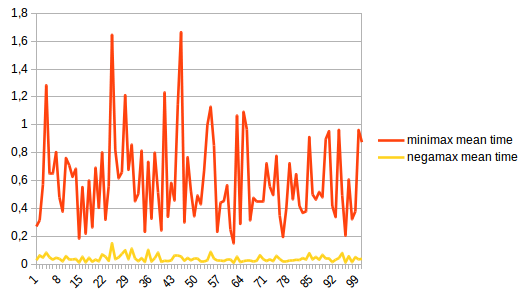
\includegraphics[scale=0.6]{temps_calcul_moyen.png}
\centering
\caption{Temps de calcul moyen sur 100 parties}
\label{graphique-temp}
\end{figure}

Le résultat illustré par ce graphique confirme ce que nous savions sur le principe alpha beta pruning. En effet, cet algorithme utilise les valeurs des noeuds déjà parcourus afin de déterminer s'il est pertinent d'explorer un nouveau noeud ou non car nous ne trouverons pas de meilleures valeurs. Ce qui nous permet de limiter le facteur de branchement de notre parcours d'arbre. Même si dans le pire des cas (La valeur de chaque noeud que l'on rencontre est plus grande que la précédente) nous aurons le même temps de parcours que notre minimax. Nous aurons dans la plupart des cas, grâce à cette optimisation la possibilité de diminuer grandement notre facteur de branchement et donc notre temps de calcul. Comme on peut encore le voir sur la figure \ref{graphique-temp}. De plus, l'atout majeur de cette optimisation est que l'on ignore aucun noeud important, ce qui nous garantit de toujours trouver le meilleur noeud de notre fonction d'évaluation.

\medbreak

Un autre moyen de réduire le facteur de branchement est de pouvoir reconnaitre les coups symétriques afin de calculer qu'une seule fois leurs valeurs au lieu d'une fois par noeud. Cependant, il ne faut pas que la recherche de noeuds symétriques nous demande plus de temps qu'elle nous ferait gagner. Nous devions donc trouver si les cas de symétrie étaient fréquents dans le jeu de reversi ou non.

Nous avions initialement prévu d'appliquer des masques de symétrie \cite{symmetry} à nos bitboards afin de repérer les situations symétriques sans avoir besoins d'utiliser de boucles pour éviter de trop augmenter notre temps de calcul.
Nous avons cependant rencontré un problème car nous utilisons des entiers de 128 bits pour pouvoir stocker une partie de 10x10 cases et nous n'avons donc pas de type assez grand pour stocker les masques dont nous avons besoins. Pour savoir si trouver une solution à ce problème aboutirait à un grand gain de temps, nous avons implémenté une détection de symétrie qui utilise une boucle pour examiner les plateaux de jeu : "Negamax\_alpha\_beta\_sym".

Nous avons donc comparé cette IA à notre version du negamax pour tester son efficacité. Malheuresement le temps de calcul était plus long avec la détection de symétrie, car on effectue une boucle de la taille du plateau à chaque nouveau noeud de l'arbre. Et en plus de l'augmentation du temps de calcul, nous détections très peu de cas de symétrie, seulement une vingtaine au maximum sur les dizaines de million de noeud que nous traitons. De plus la grande majorité de ces cas de symétrie a été trouvée dans les premiers coups de la partie et non en milieu de partie qui est la phase la plus longue pour nos IAs.

La détection de symétrie serait beaucoup plus pertinente si l'on s'en servait d'une table de hachage tout au long de la partie qui utiliserait la configuration de jeu comme clé et dans laquelle on stockerait la valeur calculée lors du premier passage dans ce noeud. En faisant en sorte que les situations symétriques amène sur la même case de la table de hachage. Cela permettrait également de ne pas recalculer à chaque tour les valeurs que l'on a trouvées lors de notre calcul du coup précedent. Il nous est cependant impossible de faire cela pour le mode "contest" du client qui implique que notre programme reparte de zéro à chaque coup que l'on cherche. Car notre programme se termine entre chaque coup et nous ne pouvons pas sauvegarder cette table.

\medbreak

Nous nous sommes aussi intéressés à d'autre technique de parcours d'arbre, tel que le "Monte Carlo\cite{MonteCarlo}". Cet algorithme est particulièrement utilisé dans les jeux où il n'y pas d'heuristique efficace connu car il peut fonctionner en sachant uniquement quand il gagne et perd une partie. Pour se faire, la valeur qu'il associe à chaque nœud est le ratio de victoire par rapport au nombre de partie qui ont déjà eu lieu en passant par ce nœud. La version de base de ce parcours d'arbre descend le plus profondément possible dans l'ensemble des nœuds déjà connus en choisissant à chaque fois le fils qui a la meilleure valeur. C'est la phase de sélection de la figure \ref{figMT}.
Une fois que le dernier nœud connu est atteint, on choisis un nouveau nœud à rajouter notre arbre, soit aléatoirement parmi les fils existants, soit en utilisant une fonction d'évaluation sur chaque fils pour estimer lequel est le plus intéressant à rajouter. C'est la phase d’expansion de la figure. Puis on simule une ou plusieurs parties à partir de ce nœud, le plus souvent en jouant aléatoirement jusqu’à arriver à une situation final. Il s'agit de la phase de simulation. Enfin, il faut remonter notre arbre pour retourner à la racine en modifiant la valeur de chaque nœud que l'on a visité. Il faut donc mettre à jour le ratio selon en conséquence du résultat de la partie simulée qui a été soit remportée, soit perdue. Cette partie est illustrée par la partie "back propagation" de la figure \ref{figMT}. Cependant, cet algorithme n'a pas de condition de fin, contrairement au minimax qui examine un nombre fini de nœuds. Il faut donc fixer un nombre de tour de boucle fini ou un temps limite de calcul.

\begin{figure}[H]
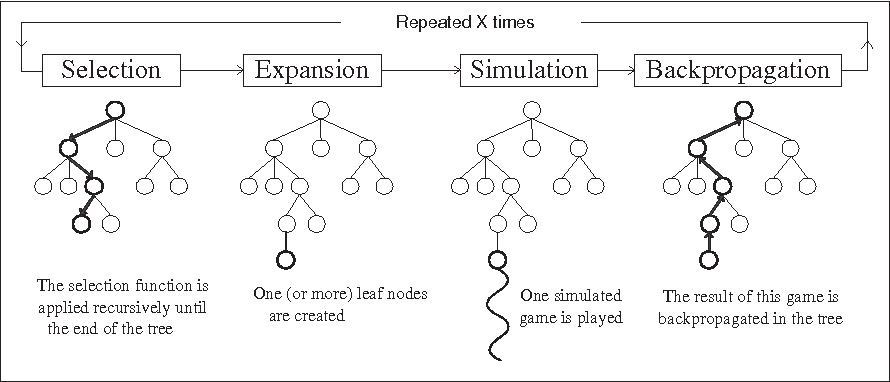
\includegraphics[scale=0.4]{MT.png}
\centering
\caption{Détails sur le principe du Monte Carlo Tree Search \cite{ChaslotMT}}
\label{figMT}
\end{figure}

Afin de tester ce parcours d'arbre, nous avons implémenté la version basique. Nous choisissons le nouveau noeud de manière aléatoire parmi les fils diponibles. Nous regardons uniquement le ratio de victoire, alors qu'il est possible d'utiliser des formules qui prennent en compte le nombre de parties jouées\cite{MonteCarlo}, ce qui pousse l'algorithme à choisir les noeuds qui ont souvent été consultés et qui ont donc un ratio plus stable. Il est également possible de simuler les parties en utilisant une fonction d'évaluation afin d'avoir des résultats plus précis.
Après avoir comparé notre IA "monte carlo" à notre IA "negamax", nous avons remarqué que le "monte carlo" avait un très faible taux de victoire. En effet, même si cette technique de parcours d'arbre est très intéressante sur des jeux complexes ou ayant différentes façon de gagner, il est nettement moins efficace qu'un parcours de l'ensemble des coups possibles qui utiliserait une fonction d'évaluation précise. Or, comme nous le savons, les heuristiques concernant le jeu de reversi sont assez précises car il y a peu de stratégies gagnantes et elles sont connues. Ce qui explique pourquoi dans notre cas, l'utilisation du "monte carlo tree search" n'est pas très perninante et c'est la raison qui nous a fait utiliser "negamax" comme algorithme de parcours d'arbre.


Enfin pour comparer nos IAs entre elles nous les avons faites affronter sur 500 parties. A partir des données récoltées nous avons créé un tableau à deux entrées contenant le pourcentage de victoire et le score moyen de chaque IAs.

\begin{table}[H]
\caption{Taux de victoire et score moyen de nos IAs (arrondi à l'entier le plus proche}
\begin{tabular}{|c||c | c | c | c | c|}
\hline
& random & basic & heuristic & neg h\_logic1 & neg h\_logic2 \\
\hline\hline
       random    	     &	X &	\backslashbox{35\% \\ 28}{62\% \\ 35} &   \backslashbox{7\% \\ 19}{92\% \\ 45}    &  \backslashbox{2\% \\ 9}{98\% \\ 51}	 &	 \backslashbox{0\% \\ 9}{100\% \\ 52}    \\
\hline
       basic   &	\backslashbox{59\% \\ 35}{37\% \\ 28} &	X & \backslashbox{9\% \\ 20}{90\% \\ 44} & \backslashbox{5\% \\ 10}{95\% \\ 50}  & \backslashbox{1\% \\ 9}{99\% \\ 52}    \\
\hline       
       heuristic   & \backslashbox{93\% \\ 43}{6\% \\ 20} & \backslashbox{88\% \\ 43}{10\% \\ 29} & X & \backslashbox{23\% \\ 20}{77\% \\ 41} & \backslashbox{9\% \\ 15}{90\% \\ 47}    \\
\hline       
       neg h\_logic1 &	\backslashbox{97\% \\ 50}{3\% \\ 9} & \backslashbox{94\% \\ 50}{6\% \\ 10} & \backslashbox{76\% \\ 42}{23\% \\ 20} &   X 	 & 	\backslashbox{18\% \\ 19}{81\% \\ 42} \\
\hline       
       neg h\_logic2 & \backslashbox{99\% \\ 53}{1\% \\ 9}	& \backslashbox{99\% \\ 53}{1\% \\ 8}&	\backslashbox{89\% \\ 47}{11\% \\ 15} & \backslashbox{74\% \\ 42}{26\% \\ 20}  &	 X \\\hline
\end{tabular}
\end{table}

En additionnant les pourcentages de victoire des deux couleurs d'une partie on n'arrive pas toujours à 100\%, cela vient du fait que certaines parties se terminent par une égalité (c'est la même chose pour la moyenne des scores qui ne fait pas 64 quand les parties s’arrête avant que toutes les cases soit occupées par un pion). La colonne de gauche correspondant au joueur ayant le premier coup (noir). Certaine IAs plus complexes peuvent perdre contre des IAs plus simples dans certains cas à cause de notre manière de générer les parties: étant générer par des IAs aléatoirement comme expliqué précédemment, un des joueur peut commencer la partie avec une configuration de plateau très désavantageuse.

Ce tableau nous montre que notre IA la plus efficace est celle utilisant un négamax en parcours d'arbre ainsi que la fonction d'évaluation h\_logic2.

\bigbreak

%TEST
%TODO test IA contre elle même -> blanc

Nous avons également réalisé un script afin d'ouvrir tous les fichiers fournis par le client et de tester notre fonction "LoadFile". Tous les fichiers s'ouvraient correctement, à l'exception du fichier du plateau 1x1. Ce qui nous à permis de nous rendre compte que l'on ne gérait pas les fins de fichier lorsque le plateau ne faisait qu'une case. Ce problème à depuis été corrigé.

Afin de tester notre IA nous avons récupéré sur internet des configurations particulières où nous connaissons le coup le plus intéressant à jouer. Grâce à un script et au mode contest nous pouvons rapidement tester toutes ces configurations et comparer le résultat donné par notre IA au coup le plus intéressant. Nous n'obtenions le même coup que sur 2 configurations sur 7. Cela vient du fait qu'il nous manque la gestion de la stabilité des pions dans le calcul de notre fonction d'évaluation.

La stabilité peut être découpée en trois sous notions:
\begin{itemize}
\item Les pions stables: qui ne pourront plus être retournés
\item Les pions instables: qui peuvent être retournés au prochain coup de l'adversaire
\item Les pions semi-stables: qui ne peuvent pas être retournés au prochain coup mais pourrait être retournés plus tard dans la partie
\end{itemize}

Nous avons aussi pensé à faire jouer nos IAs contre elle même et voir quelle couleur gagné. En effet le fait de commencer ou de jouer en second donne souvent un avantage minime dans les jeux de plateau, d'après nos recherche au reversi ce serai le joueur blanc qui aurait l'avantage car il pose le dernier pion. Cependant cette stratégie ne fonctionne pas très bien en pratique car cette avantage s'inverse à chaque fois qu'un joueur doit passer son tour.

\section{Conclusion}

Nous avons réussi à créer une IA capable de battre un joueur expérimenté. Selon les algorithmes de parcours d'arbre utilisés, nous pouvons explorer à environ 9 de profondeur en milieu de partie. Il pourrait cependant être intéressant de pouvoir faire varier la profondeur de parcours d'arbre. Les débuts et fins de partie se calculent plus rapidement que le milieu de partie car il y a moins de coups possible. Varier la profondeur nous permettrait d'utiliser au mieux la limite de temps de calcul que nous avons.

Afin d'améliorer notre heuristique se basant sur les connaissances du jeu et ainsi augmenter nos chances de victoire contre un adversaire pouvant aller à une profondeur équivalente à la notre il nous faudrait inclure la notion de stabilité un élément stratégique presque aussi important que les coins.

Pour améliorer la rapidité de nos parcours d'arbre il serait intéressant de les multithreader, c'est une optimisation difficile à mettre en place car l'optimisation alpha-béta prunning implique que l'on parcourt les noeuds dans l'ordre or nous n'avons pas cette garantie si l'on parallélise notre parcours d'arbre. Il nous faudrait trouver un moyen de communiquer aux autres threads les branches moins intéressantes que la notre pour ne pas la parcourir.

Enfin nous pourrions nous inspirer d'AlphaGo Zero et implémenter un algorithme utilisant le machine learning de façon à développer une IA apprenant d'elle même sans avoir besoin de notre heuristique logique.

\section{Bibliographie}

\bibliographystyle{unsrt}
\bibliography{biblio}
\end{document}